%=============================================================================%
% Author: 	John Joseph Valletta
% Date: 	23/04/2017
% Title: 	Python workshop: Matplotlib
%=============================================================================%

%=============================================================================%
% Preamble
%=============================================================================%
% Libraries
\documentclass[pdf]{beamer}
\usepackage[export]{adjustbox}
\usepackage{framed}
\usepackage{color}
\definecolor{dkgreen}{rgb}{0,0.6,0}
\definecolor{gray}{rgb}{0.5,0.5,0.5}
\definecolor{mauve}{rgb}{0.58,0,0.82}
\definecolor{deepblue}{rgb}{0,0,0.5}
\definecolor{deepred}{rgb}{0.6,0,0}
\definecolor{deepgreen}{rgb}{0,0.5,0}
\definecolor{lightgray}{rgb}{0.92,0.92,0.92}
\usepackage{listings} % to insert code
\usepackage{textpos} % textblock
\usepackage{dirtree} % to make directory trees
\usepackage{hyperref}
\hypersetup{colorlinks=true, urlcolor=blue, linkcolor=black} 

% Listing set up
% Python
\lstdefinestyle{python}{
language=python,
formfeed=\newpage,
basicstyle=\scriptsize\ttfamily,
commentstyle=\color{deepgreen},%\color{gray},
%numbers=left,
%numberstyle=\tiny\color{gray},
stepnumber=1,
numbersep=5pt,
backgroundcolor=\color{lightgray},%\color{white},
showspaces=false,
showstringspaces=false,
showtabs=false,
frame=lines,
tabsize=4,
captionpos=b,
breaklines=true,
breakatwhitespace=false,
title=\lstname,
escapeinside={},
keywordstyle=\color{deepblue},
emphstyle=\color{deepred},
stringstyle=\color{mauve},
morekeywords={as, lambda, None}
}

% Presentation configuration
\mode<presentation>{\usetheme{Madrid}}
\definecolor{tealblue}{rgb}{0, 0.5, 0.5}
\usecolortheme[named=tealblue]{structure}
\useinnertheme{circles} % circles, rectanges, rounded, inmargin
\usefonttheme[onlymath]{serif} % makes math fonts like the usual LaTeX ones
\setbeamercovered{transparent=4} % transparent
\setbeamertemplate{caption}{\raggedright\insertcaption\par} % Remove the word "Figure" from caption %\setbeamertemplate{caption}[default]
\setbeamertemplate{navigation symbols}{} % don't put navigation tools at the bottom (alternatively \beamertemplatenavigationsymbolsempty)
\graphicspath{ {../images/} }

% Titlepage
\title[Python for scientific research]{Python for scientific research}
\subtitle{Plotting with \texttt{Matplotlib}}
\author{John Joseph Valletta}
\date[June 2017]{June 2017}
\institute[]{University of Exeter, Penryn Campus, UK}
\titlegraphic{
\hfill

\includegraphics[width=\textwidth, keepaspectratio]{logo.jpg}}

%=============================================================================%
%=============================================================================%
% Start of Document
%=============================================================================%
%=============================================================================%
\begin{document}

%=============================================================================%
%=============================================================================%
\begin{frame}
\titlepage
\end{frame}

%=============================================================================%
%=============================================================================%
\begin{frame}{What we've done so far}

	\begin{enumerate}\addtolength{\itemsep}{1\baselineskip}
		\item Declare variables using built-in data types and execute operations
		on them
		\item Use flow control commands to dictate the order in which commands are run
		and when
		\item Encapsulate programs into reusable functions, modules and packages
		\item Using \texttt{NumPy} and \texttt{SciPy} for numerical computations
		\item \textbf{Next}: Introducing \texttt{Matplotlib}, Python's plotting library
	\end{enumerate}

\end{frame}

%=============================================================================%
%=============================================================================%
\begin{frame}{Introduction}

\begin{itemize}
	\item \texttt{Matplotlib} is a 2D and 3D plotting library that produces
	publication-ready scientific figures in most formats (e.g PNG, EPS)
\end{itemize}

\begin{center}
	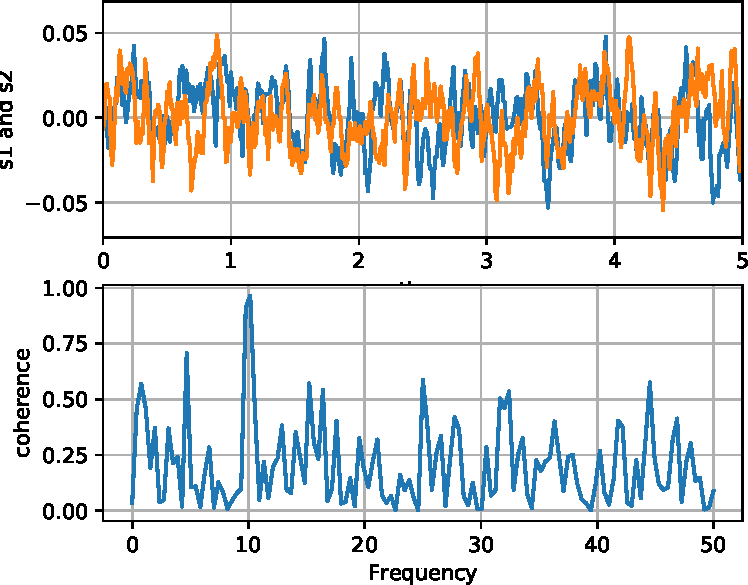
\includegraphics[width=.3\textwidth]{demo1.pdf}\hfill
	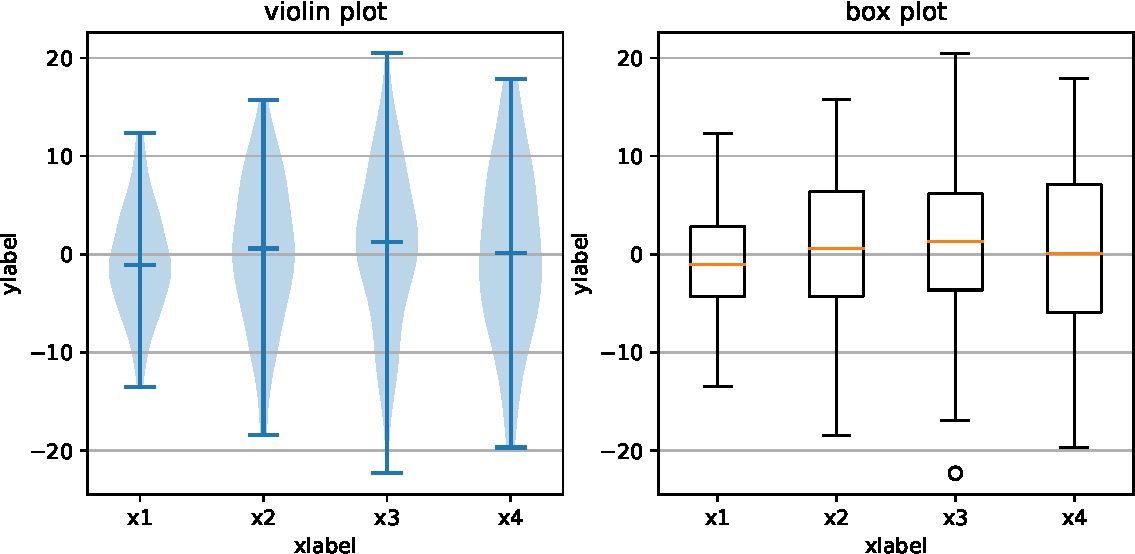
\includegraphics[width=.42\textwidth]{demo5.pdf}\hfill
	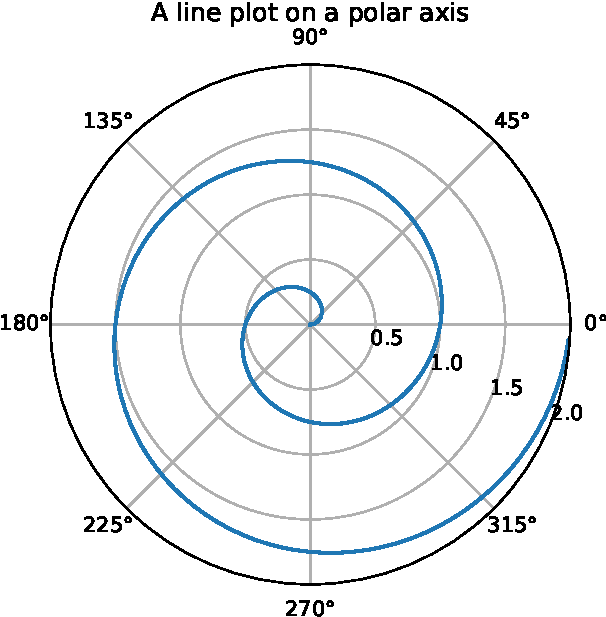
\includegraphics[width=.22\textwidth]{demo3.pdf}\\
	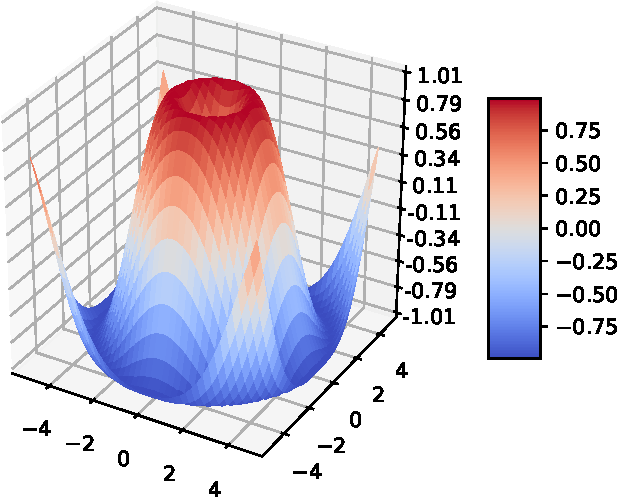
\includegraphics[width=.32\textwidth]{demo4.pdf}\hfill
	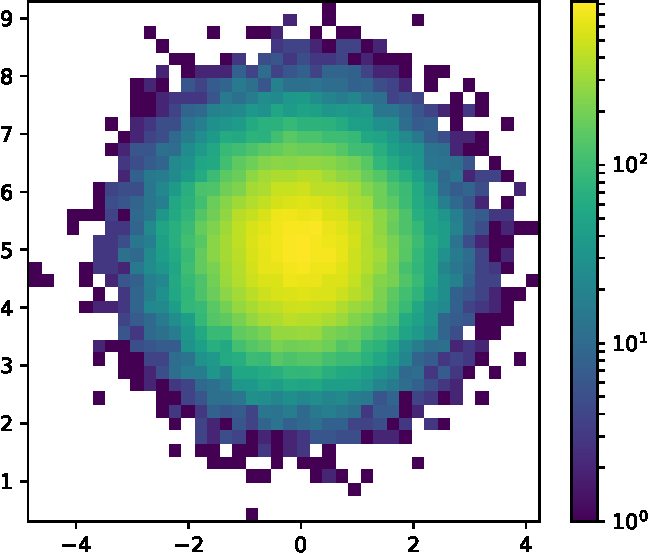
\includegraphics[width=.28\textwidth]{demo2.pdf}\hfill
	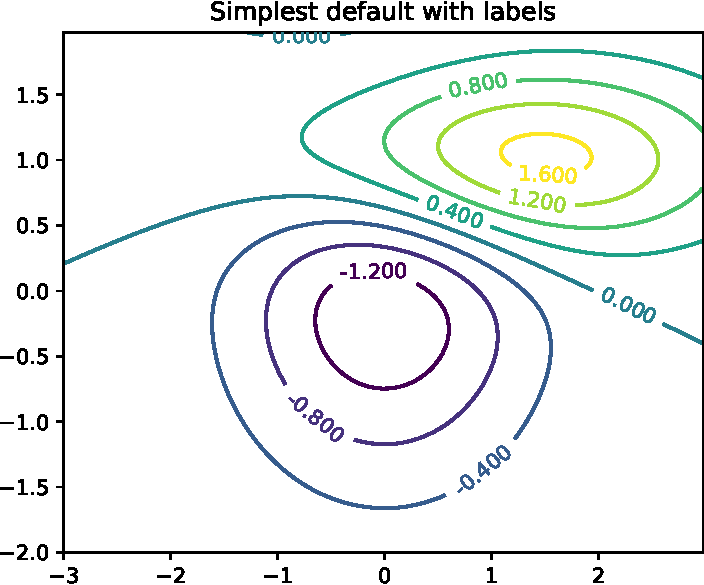
\includegraphics[width=.3\textwidth]{demo6.pdf}
\end{center}
\end{frame}

%=============================================================================%
%=============================================================================%
\begin{frame}{Anatomy of a figure}

\begin{center}
	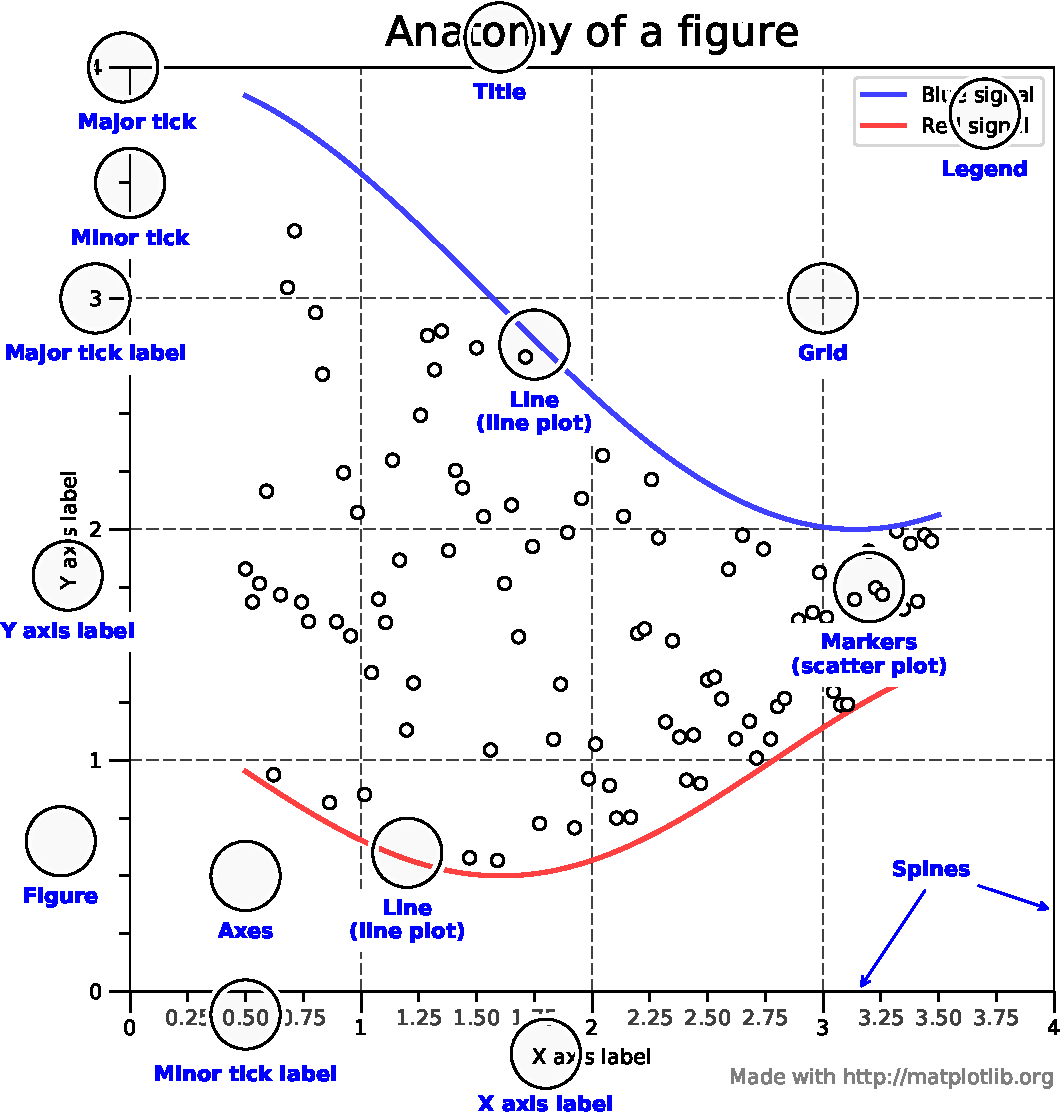
\includegraphics[width=.6\textwidth]{anatomy_figure.pdf}
\end{center}
\end{frame}

%=============================================================================%
%=============================================================================%
\begin{frame}[fragile]
\frametitle{My first plot}

\begin{lstlisting}[style=python]
import numpy as np
import matplotlib.pyplot as plt

# Generate a sinusoidal data
x = np.linspace(0, 4*np.pi, 100)
y = np.sin(x)

# Plot sinusoidal curve
plt.plot(x, y, color="blue")
plt.xlabel("Time")
plt.ylabel("Amplitude")
plt.title("My first Python plot")
\end{lstlisting}

\vspace{-0.5cm}
\begin{center}
	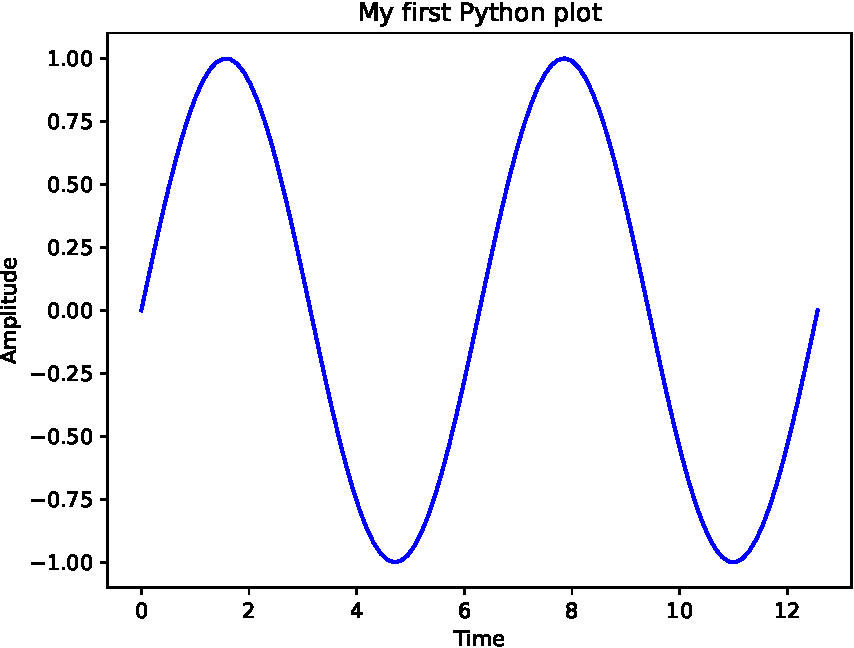
\includegraphics[width=.35\textwidth]{plot1.pdf}
\end{center}

\end{frame}

%=============================================================================%
%=============================================================================%
\begin{frame}[fragile]
\frametitle{Subplots}

\begin{lstlisting}[style=python]
plt.subplot(2, 1, 1) # 2 rows, 1 column, first plot
plt.plot(x, np.sin(x), color="b", label="Sine")
plt.ylabel("Amplitude")
plt.legend(loc="upper right")

plt.subplot(2, 1, 2) # 2 rows, 1 column, second plot
plt.plot(x, np.cos(x), color="r", label="Cosine")
plt.xlabel("Time")
plt.ylabel("Amplitude")
plt.legend(loc="upper right")
\end{lstlisting}

\vspace{-0.5cm}
\begin{center}
	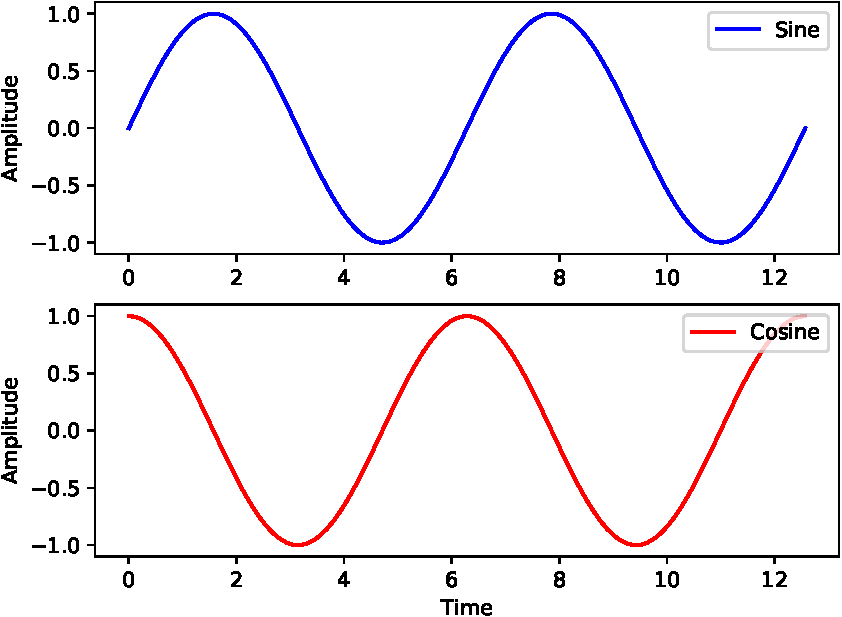
\includegraphics[width=.4\textwidth]{plot2.pdf}
\end{center}

\end{frame}

%=============================================================================%
%=============================================================================%
\begin{frame}[fragile]
\frametitle{Histograms}

\begin{lstlisting}[style=python]
# Generate 1000 normally distributed numbers
x1 = np.random.randn(1000) 
x2 = np.random.randn(1000) 

# 1D histogram (x1)
plt.subplot(1, 2, 1)
plt.hist(x1, bins=20)

# 2D histogram (x1 vs x2)
plt.subplot(1, 2, 2)
plt.hist2d(x1, x2, bins=20)
plt.colorbar()
\end{lstlisting}

\vspace{-0.6cm}
\begin{center}
	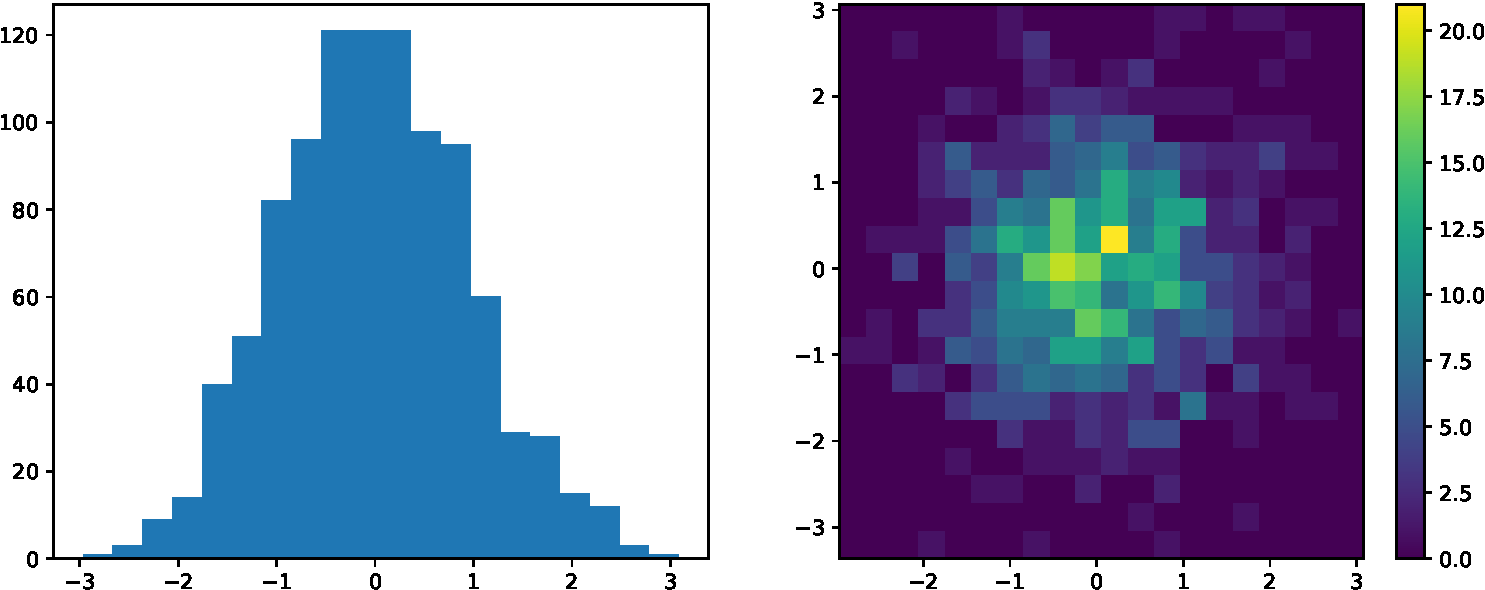
\includegraphics[width=.72\textwidth]{plot3.pdf}
\end{center}

\end{frame}

%=============================================================================%
%=============================================================================%
\begin{frame}[fragile]
\frametitle{Boxplots and violin plots}

\begin{lstlisting}[style=python]
# Generate four sets of random numbers
data = [np.random.randn(1000) for i in range(4)]

# Boxplot
plt.subplot(1, 2, 1)
plt.boxplot(data)

# Violin plot
plt.subplot(1, 2, 2)
plt.violinplot(data)
\end{lstlisting}

\vspace{-0.6cm}
\begin{center}
	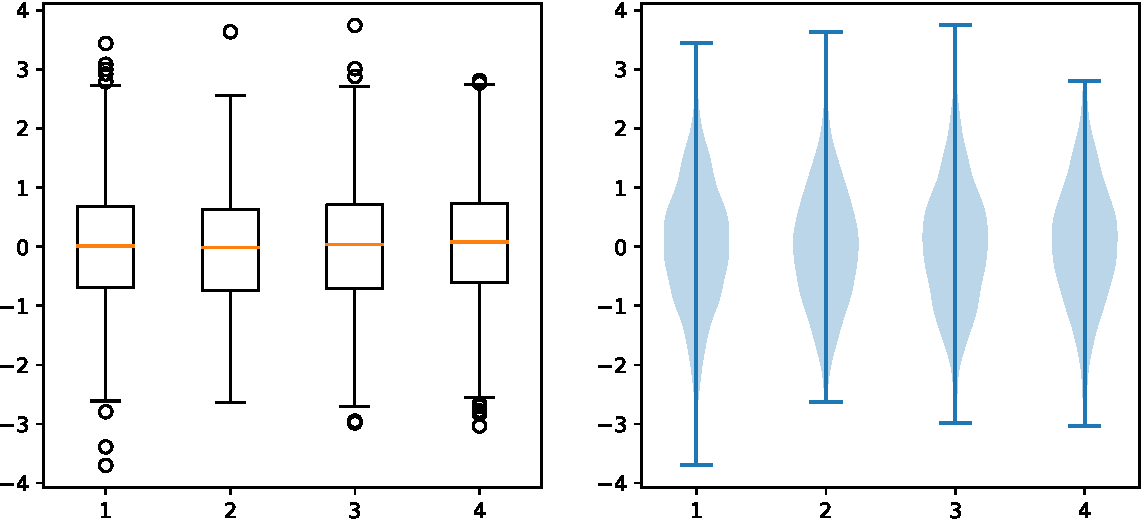
\includegraphics[width=.72\textwidth]{plot4.pdf}
\end{center}

\end{frame}

%=============================================================================%
%=============================================================================%
\begin{frame}[fragile]
\frametitle{Contour plot}

\tiny
\begin{lstlisting}[style=python]
from matplotlib import cm

# Generate some x, y, z data
x = np.arange(-2.5, 2.5, 0.1)
y = np.arange(-2.5, 2.5, 0.1)
x, y = np.meshgrid(x, y)
z = np.exp(-x**2 - y**2)

# Contour plot
plt.contourf(x, y, z, cmap=cm.inferno)
plt.colorbar()
\end{lstlisting}

\vspace{-0.8cm}
\begin{center}
	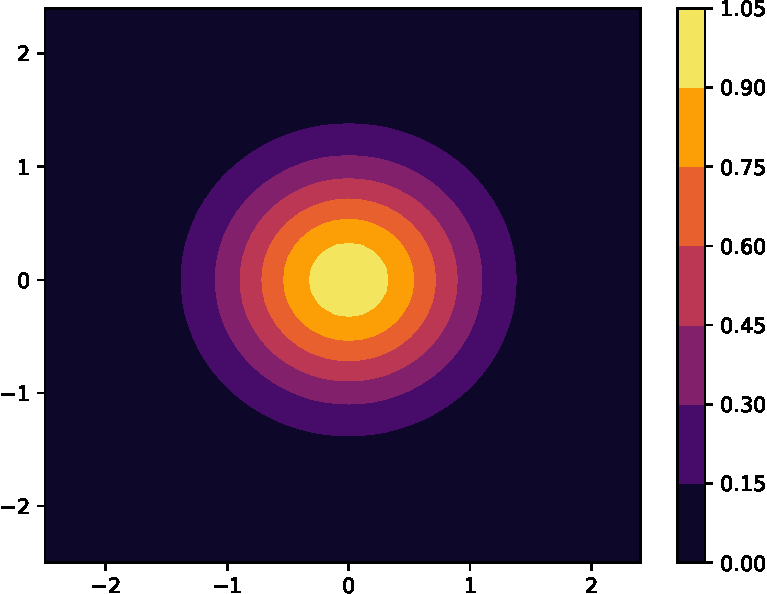
\includegraphics[width=.42\textwidth]{plot5.pdf}
\end{center}

\end{frame}

%=============================================================================%
%=============================================================================%
\begin{frame}[fragile]
\frametitle{3D surface}

\tiny
\begin{lstlisting}[style=python]
from mpl_toolkits.mplot3d import Axes3D

# Create figure amenable for 3D plotting
hFig = plt.figure()
hAx = hFig.gca(projection="3d")

# Plot the surface
hSurf = hAx.plot_surface(x, y, z, cmap=cm.inferno)
plt.colorbar(hSurf, shrink=0.5)
\end{lstlisting}

\vspace{-0.8cm}
\begin{center}
	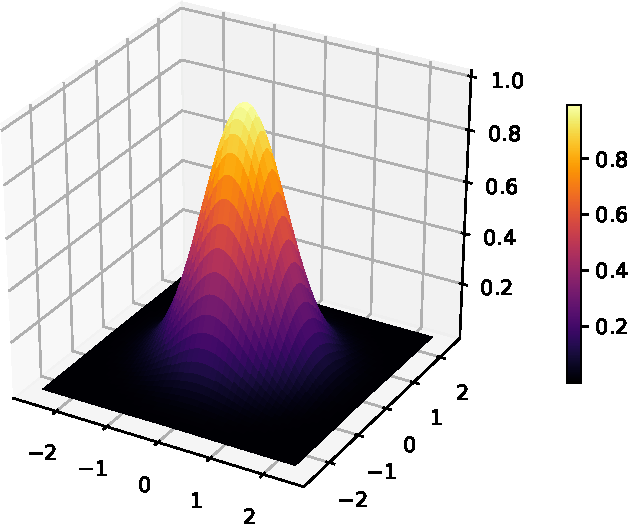
\includegraphics[width=.42\textwidth]{plot6.pdf}
\end{center}

\end{frame}

%=============================================================================%
%=============================================================================%
% End of Document
%=============================================================================%
%=============================================================================%
\end{document}
